\section{Ergebnisse der Anordnungsvariation}\label{anhang:Anordnung}
In diesem Abschnitt werden die Ergebnisse der Variation der Anordnung dargestellt, die im Verlauf der Arbeit nicht weiter ausgearbeitet wurden. Der Einfluss erscheint für den späteren Einsatz nicht relevant.\\
Aus Abbildung~\ref{fig:fieldAnordnung} geht die Feldverdrängung im Ringkern hervor, die durch die Kurzschlüsse verursacht wird. Es ist zu sehen, dass ein breiter Kurzschluss weniger Feld verdrängt als zwei schmalere. Dies spiegelt sich auch in den Ergebnissen der Simulation wieder, die in Abbildung~\ref{fig:simAnordnung} dargestellt ist.\\
Der Einfluss der Anordnung spielt generell mit der verwendeten und simulierten Testbox eine größere Rolle als dies in einer Kavität der Fall sein sollte. Dies wird in den Abbildungen~\ref{fig:fieldAnordnung} und~\ref{fig:simAnordnung} deutlich, da hier die Anordnung von zwei gegenüberliegenden Kurzschlüssen eine bessere Verringerung der Ringkernimpedanz liefert, als wenn die Kurzschlüsse nebeneinander angeordnet werden. Dies ist dem im Bezug auf den Ringkern nicht zentral gelagerten Einkopplungsrohr zugrunde zu legen, in einer Kavität befindet sich das Strahlrohr zentrisch bezogen auf den Ringkern.

\begin{figure}[htb]
    \centering
    \subfloat[1 Kurzschluss, Breite $\SI{30}{\milli\meter}$]{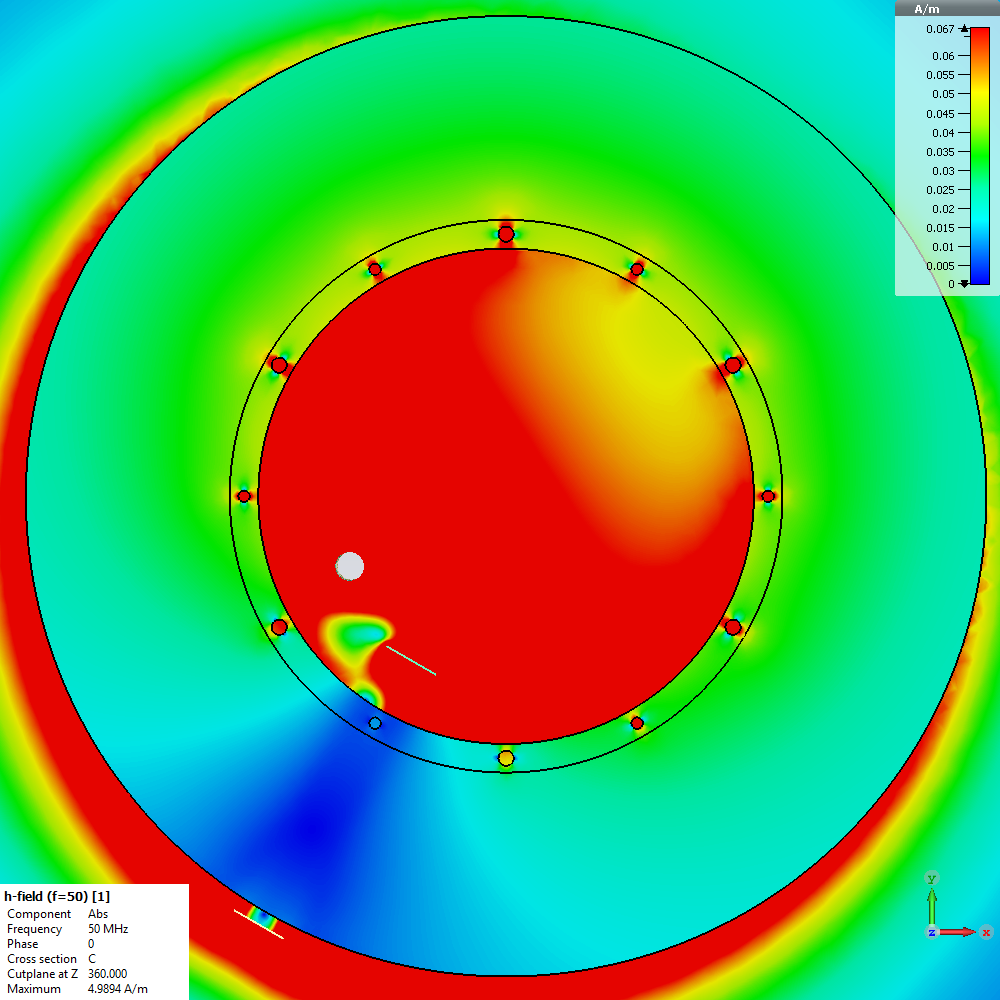
\includegraphics[width=0.33\textwidth]{Feldbilder/1KS}}
    \subfloat[2 Kurzschl\"usse gegenüber, Breite $\SI{30}{\milli\meter}$]{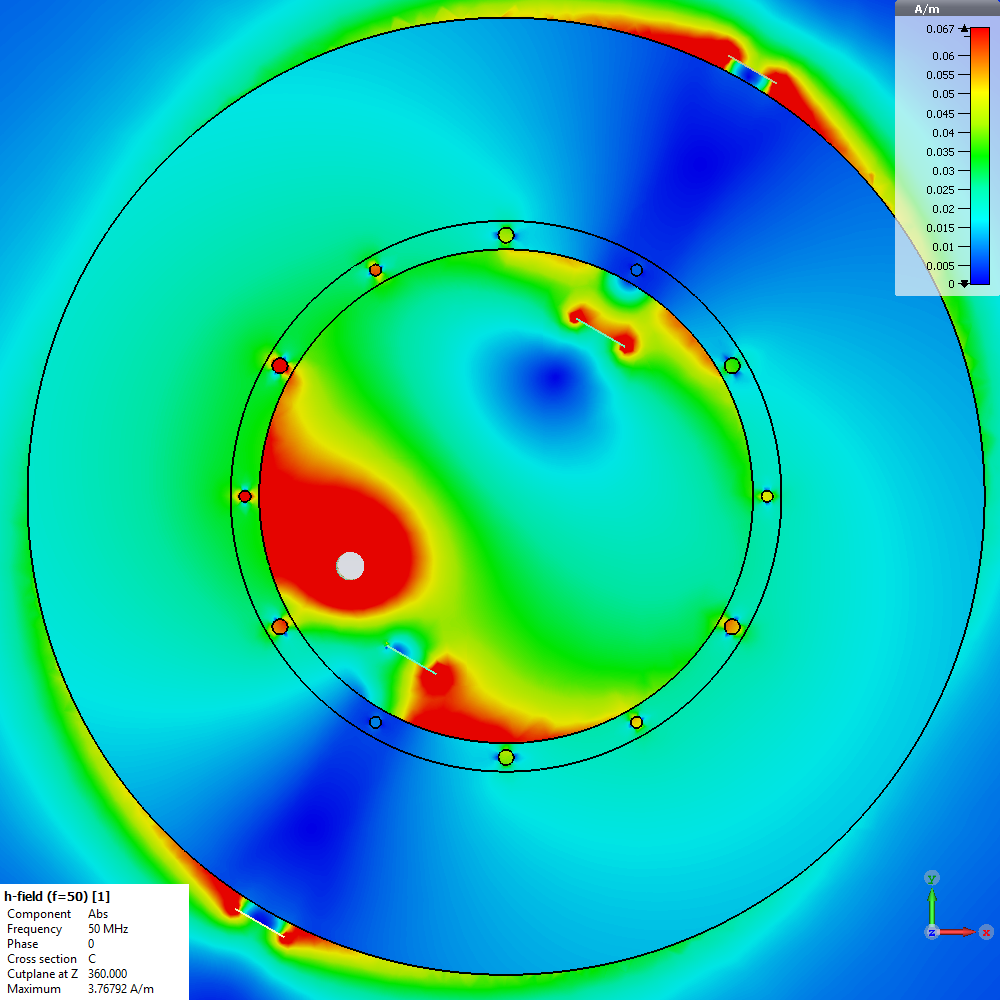
\includegraphics[width=0.33\textwidth]{Feldbilder/2KS}}\\
    \subfloat[2 Kurzschlüsse nebeneinander, Breite $\SI{30}{\milli\meter}$]{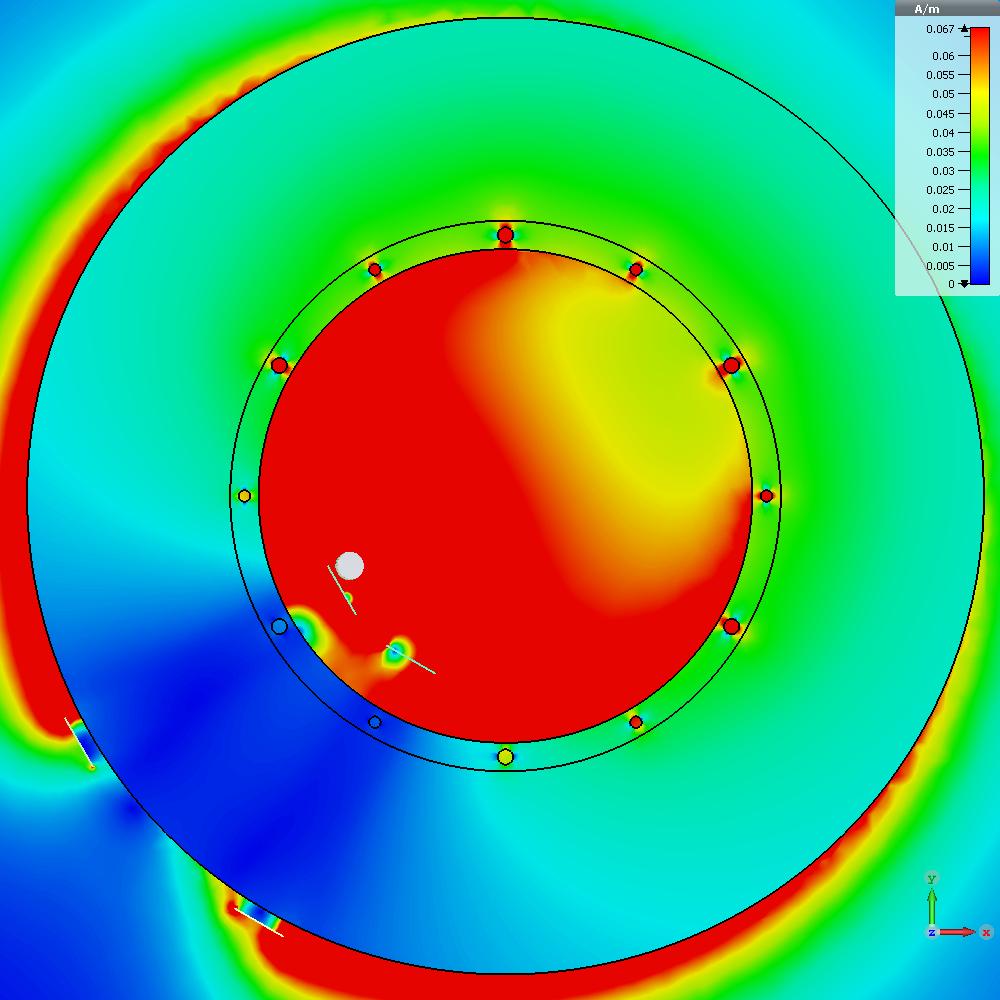
\includegraphics[width=0.33\textwidth]{Feldbilder/2KSnah}}
    \subfloat[1 Kurzschluss, Breite $\SI{50}{\milli\meter}$]{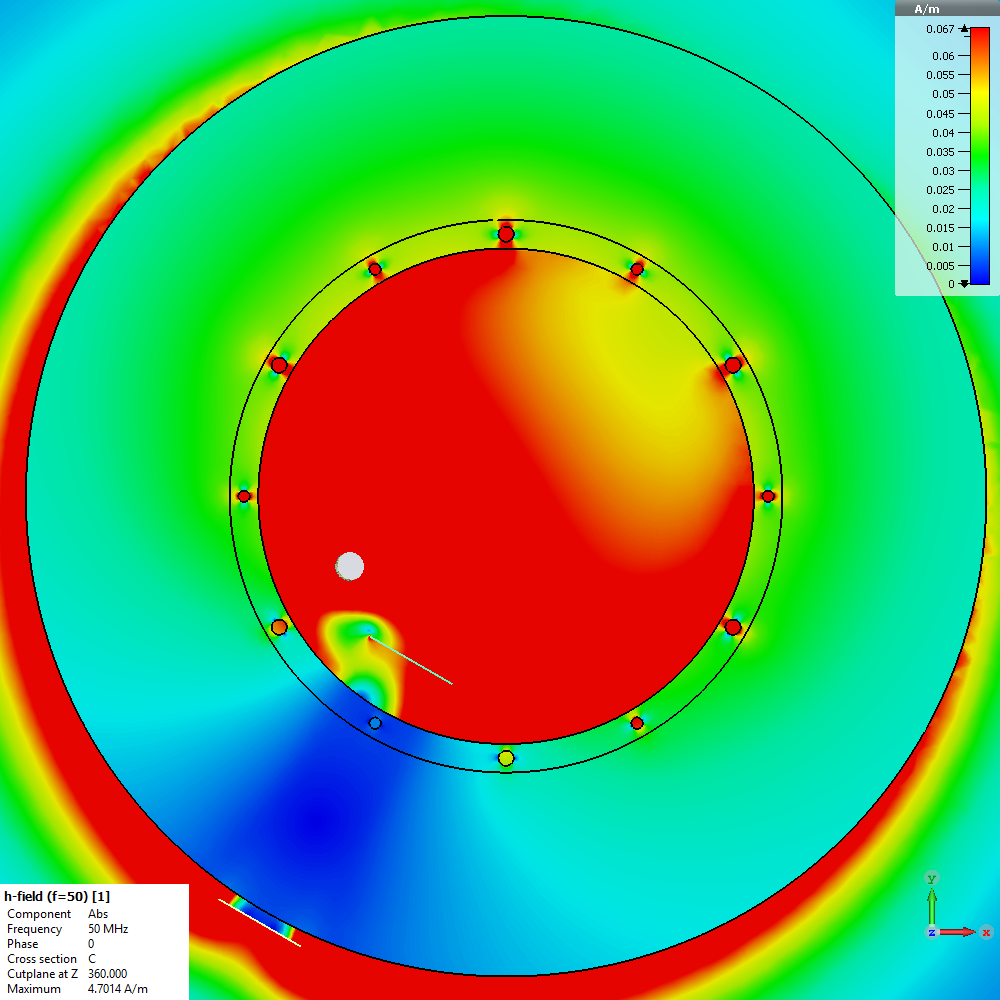
\includegraphics[width=0.33\textwidth]{Feldbilder/1KSb50}}
    \caption{Gegen\"uberstellung der Feldbilder für die Variation der Anordnung von Kurzschlüssen um den Ringkern.}
    \label{fig:fieldAnordnung}
\end{figure}

\begin{figure}[htb]
    \centering
    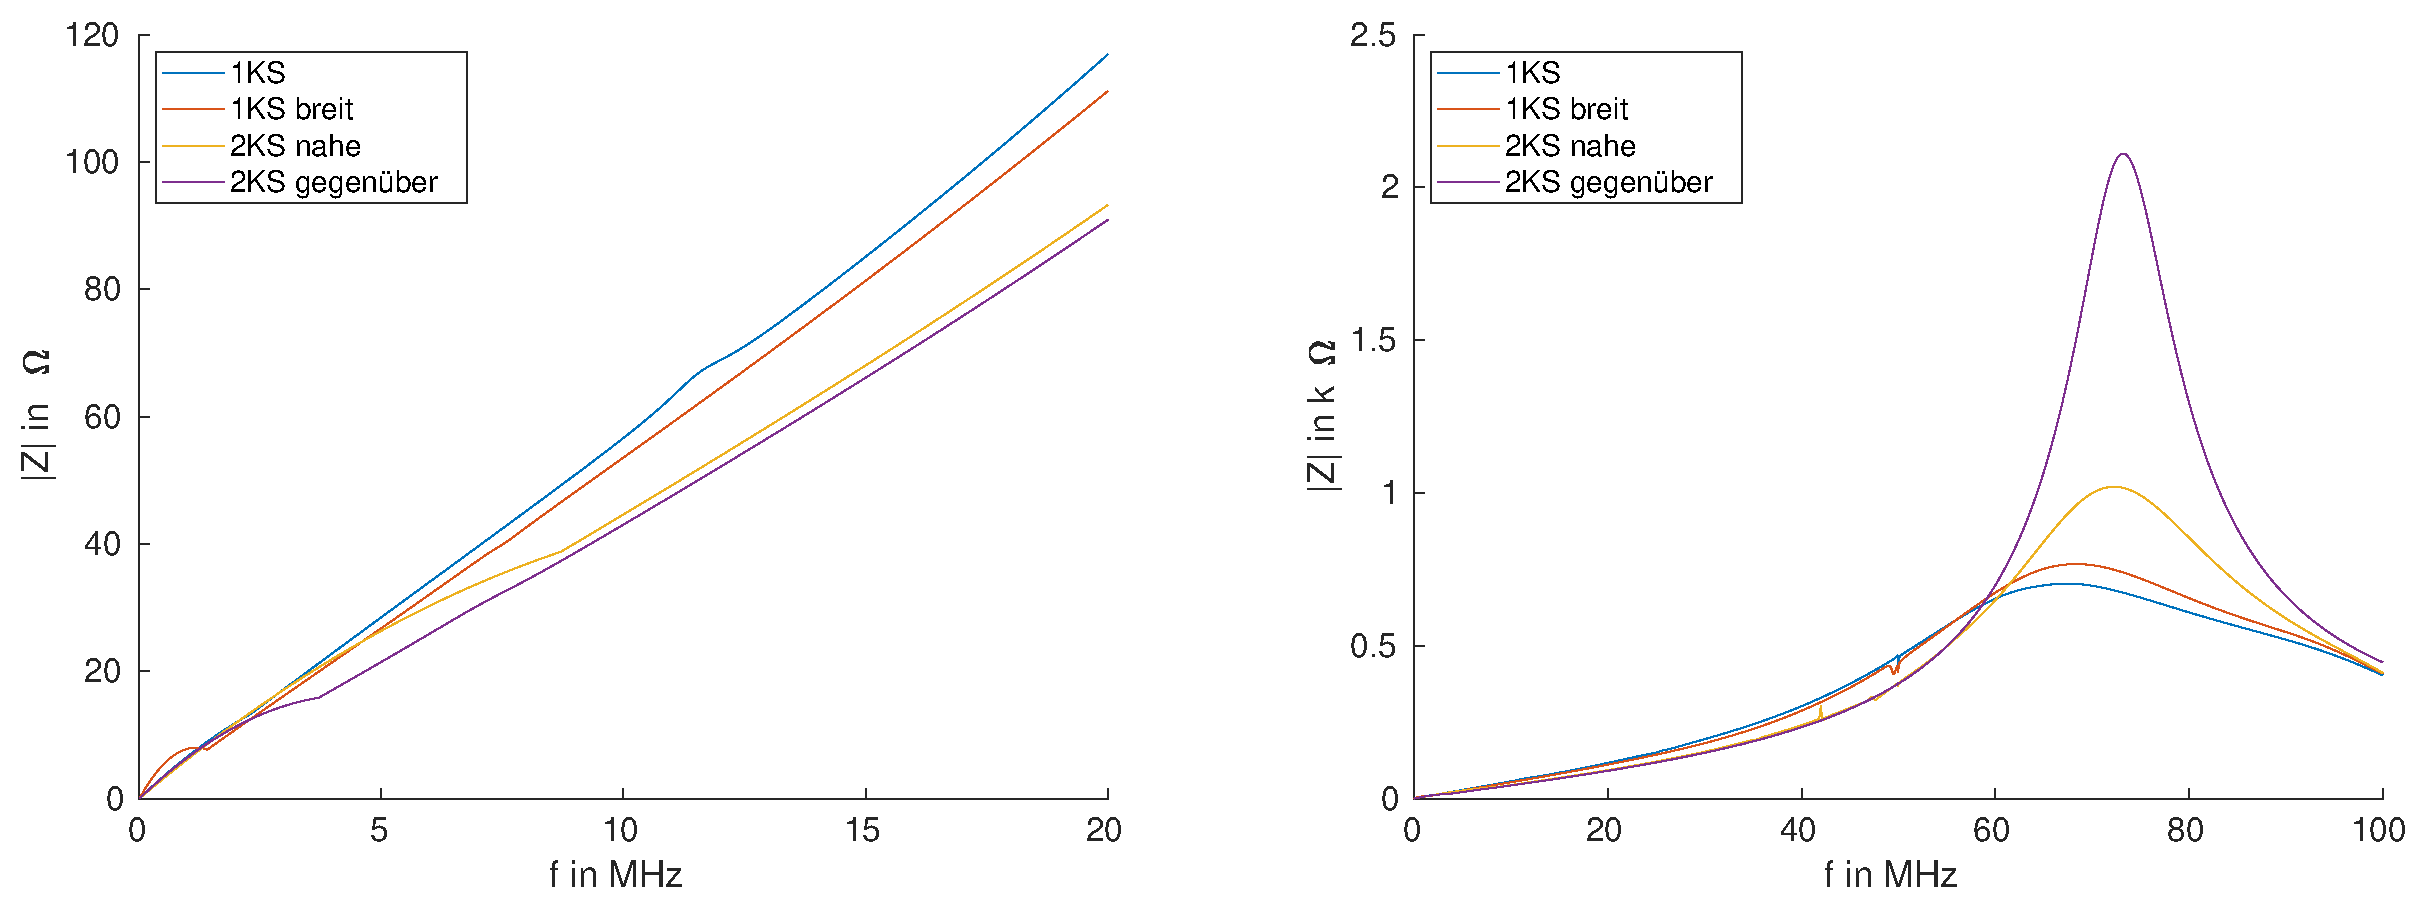
\includegraphics[width=\textwidth]{Z_ges_KSnahe_gegen}
    \caption{Simulationsergebnisse für die Variation der Anordnung von Kurzschlüssen um den Ringkern.}
    \label{fig:simAnordnung}
\end{figure}
